\documentclass[11pt]{article}
\usepackage[margin=20mm]{geometry}
\usepackage{booktabs,graphicx,hyperref}
\begin{document}
\title{Event analysis: ion production and diffusion}
\author{NAUSICAA}\date{}\maketitle
This checkpoint implements Petit's per-hit rounding and per-ion Gaussian Monte
Carlo histogram, with explicit RNG inputs, Float32 physical arrays, Int64 counts,
saved edges and a charge ledger. The cumulative Julia suite passes 1953 assertions.
The pinned replay fixture agrees with Petit's original Float64 diffusion routine
away from bin boundaries. Geometry, conservation, stochastic moments, finite-window
losses, exact edges and reproducibility have separate tests.

\section*{Model and numerical conventions}
The mean pair-creation energy is 21.9 eV. Counts are rounded independently per
hit, with ties to even. The model uses a common drift distance per event, sampled
uniformly from the configured interval. The thermal-width formula retains Petit's
$k_B/e=8.6173\times10^{-5}$ V/K, at 293.15 K and 200 V/cm. The baseline uses
the same width on all axes. The zero-longitudinal-width comparison is supported.
Coordinates remain in the source frame.

Histogram bounds span the hit extent plus the configured sigma padding. Internal
bins are half open; the final upper edge is included. A coincident axis with zero
diffusion uses one bin centred at that coordinate and adjacent representable
Float32 edges. Every ion consumes three Gaussian draws. Outside counts remain in
the ledger; retained counts are never renormalised. Int64 counts satisfy
$N_{\rm sampled}=N_{\rm retained}+N_{\rm outside}$ exactly.

\section*{Full-sample ion production}
\begin{center}\small\begin{tabular}{lrrrr}\toprule
Sample & Events & Mean rounding [ions] & Max rounding [\%] & Max arithmetic error \\\midrule
Double beta & 8995 & 0.60 & 0.0172 & 2.57e-07 \\
Electron background & 8483 & 0.56 & 0.0172 & 3.27e-07 \\
\bottomrule\end{tabular}\end{center}
Rounding means sampled minus expected ions. The maximum rounding column uses
the absolute event-relative difference. Arithmetic error compares Float32 ion
expectations with an independent Float64 E/W sum; it is a relative error.

\section*{Diffusion checks}
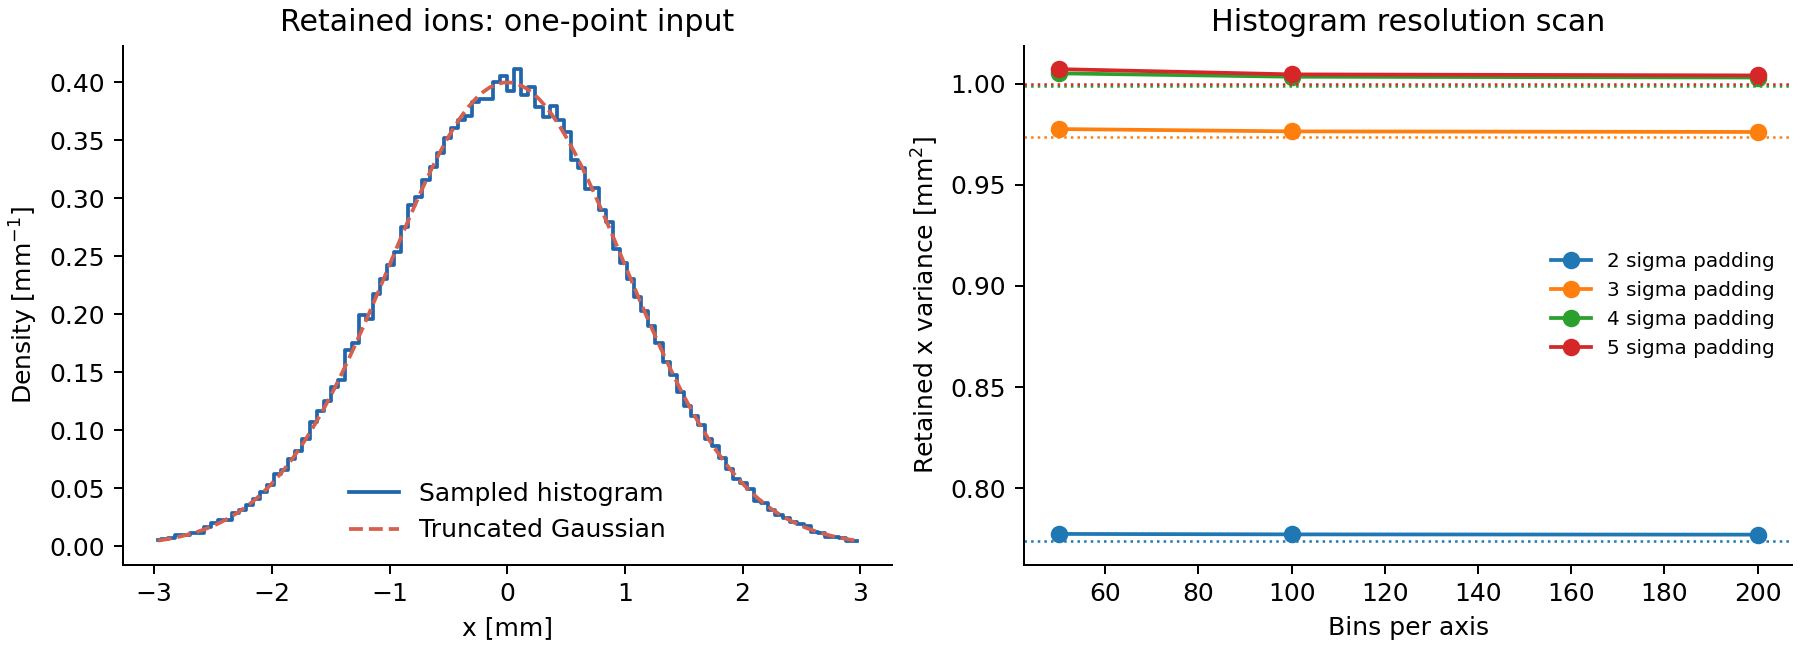
\includegraphics[width=\linewidth]{diffusion_validation.png}
The point-source example has sigma=1 mm. The right panel compares retained
histogram-centre variance with the analytic truncated-Gaussian variance (dotted
lines). The same Gaussian draws are replayed at every bin count and padding.
Increasing padding recovers the Gaussian tails; changing bin count preserves
the retained count for fixed bounds. Finite-sample fluctuations remain after
the histogram resolution converges.

\begin{center}\begin{tabular}{rrrr}\toprule
Padding [sigma] & Sampled ions & Outside ions & Analytic outside [\%] \\\midrule
2 & 200000 & 26043 & 13.038 \\
3 & 200000 & 1615 & 0.80775 \\
4 & 200000 & 32 & 0.019002 \\
5 & 200000 & 0 & 0.00017199 \\
\bottomrule\end{tabular}\end{center}

\begin{center}\begin{tabular}{lrrr}\toprule
Sample & Cases & Mean diffusion [ms] & Max outside [\%] \\\midrule
Double beta & 20 & 6.55 & 0.0321 \\
Electron background & 20 & 5.99 & 0.0205 \\
\bottomrule\end{tabular}\end{center}
The real-event checks cover events spread across each file, at the configured
fixed drift distances and one sampled distance per event. Timings include histogram
allocation and output construction after compilation; measured values depend on
the machine. The HDF5 also records allocated bytes and seeds. These checks
establish the diffusion stage. Selection efficiencies and pad histories belong
to the next integration checkpoint.

\section*{Reproduction}
\begin{verbatim}
make validate-event-step2 PYTHON=/path/to/python3.11-or-newer
# Regenerate presentation from saved HDF5:
make report-event-step2 PYTHON=/path/to/python3.11-or-newer
\end{verbatim}
Source hashes, resolved inputs and measured tables are saved in:
\par\noindent\path{results/event_analysis/step2_validation.h5}.
\par
The HTML review contains the implemented signatures and source docstrings.
\section*{Configuration used}
\small\begin{verbatim}
# Ion-production/diffusion checkpoint. Detector constants come from the SI card.
[inputs]
detector_card = "config/detector.toml"
samples = ["events/0nubb_hitdf.h5", "events/electron_0nubb_energy_hitdf.h5"]

[ionization]
ionisation_energy_eV = 21.9
# Same adopted nominal W as the initial ion_tracks analysis.

[drift]
min_cm = 10.0
max_cm = 150.0

[diffusion]
longitudinal = "thermal" # "zero" is the longitudinal comparison
nbins = 100
nsigma = 3.0

[graph]
# Approved settings for the next integration stage.
method = "kNN"
k = 10
min_ions_per_bin = 10
bin_sigma_scale = 3.0
edge_sigma_scale = 6.0

[random]
seed = 2026
# Validation uses explicit per-case seeds, stored in its HDF5.

[validation]
events_per_sample = 5
synthetic_ions = 200000
drift_cm = [10.0, 80.0, 150.0]
bin_counts = [50, 100, 200]
padding_sigma = [2.0, 3.0, 4.0, 5.0]

\end{verbatim}
\end{document}
